% master file siminos/froehlich/slice/FrCv11.tex    pdflatex FrCv11
% $Author$ $Date$

                        %% logical setup, no need to edit %%%%%%%%%%
                        \newif\ifpaper \newif\ifPDF               %%
                        \newif\ifboyscout  \newif\ifarticle       %%
                        \boyscouttrue %% commented, WWW/boyscouts %%
                        \articlefalse %% journal submission		  %%
                        \paperfalse\PDFtrue %% hyperlinked    %%%%%%
%%% Toggle between draft and non-draft versions
%\boyscoutfalse                 % public, hyperlinked for our homepages
%\articletrue 					% article for submission
								% uses \documentclass[preprint,12pt]

%%   based on Elsavier/elsarticle-template-3-num.tex, ver. 165 2009-10-08
% Predrag, reformatted for CNSNS				2011-01-02
%%   abandoned initial aiptemplate.tex AIP REVTeX4 Ver. 4.1
% Predrag, created the first draft				2010-11-21


%% ------------------ for arXiv submission ----------------------------
%
% Title:    Reduction of continuous symmetries of chaotic flows
%           by the method of slices
% Authors:  Stefan Froehlich and Predrag Cvitanovic
% Comments: submitted to
%		    "Comm. Nonlinear Sci. and Numerical Simulation"
% 			? pages, ? postscript figures,
%			uses elsarticle.cls, numcompress.sty
% Files:    FrCv11.tex FrCv11Defs.tex FrCv11.bbl
%           ??.png ??.png  ??.png
%
%% ------------------ cut here ----------------------------------------

	\ifarticle
\documentclass[preprint,12pt]{elsarticle} % submit this to journal
\papertrue\boyscoutfalse
	\else
\documentclass[final,3p,times,sort&compress]{elsarticle}	% journal layout
	\fi
%% Use the option review to obtain double line spacing
%% \documentclass[preprint,review,12pt]{elsarticle}


%\draft %obsolete, invoke option instead
% marks overfull lines with a black rule on the right
\usepackage{amssymb}
\usepackage{amsmath}
\usepackage{graphicx}
	\ifarticle\else
\usepackage[pdftex,colorlinks]{hyperref}
	\fi
%% The numcompress package shorten the last page in references.
%% `nodots' option removes dots from firstnames in references.
\usepackage[nodots]{numcompress}

\input ./defsFrCv11            %% FrCv11 macros
\graphicspath{{../../figs/}{../../Fig/}}  %% directories with color graphics files
\journal{Communications in Nonlinear Science and Numerical Simulation}
\begin{document}
\title{Reduction of continuous symmetries of chaotic flows
       by the method of slices}
% earlier titles:
% "Reduction of continuous symmetries by the method of slices"

\author{Stefan Froehlich}

\author{Predrag Cvitanovi\'{c}\corref{cor1}}
\ead{predrag@gatech.edu}
\cortext[cor1]{Corresponding author}
\ead[url]{ChaosBook.org}

\address{Center for Nonlinear Science,
        School of Physics, Georgia Institute of Technology,
        Atlanta, GA 30332-0430}

\date{\today}

\begin{abstract}
% former file siminos/froehlich/slice/abstract.tex 2011-01-13
  %
We study continuous symmetry reduction of dynamical systems
by the \mslices\ (\mframes) and show that a `slice'
defined by minimizing the distance to a single generic `{\template}'
intersects the group orbit of every point in the full {\statesp}. Global
symmetry reduction by a single slice is, however, not natural for a
chaotic / turbulent flow; it is better to cover the \reducedsp\ by a set
of slices, one for each dynamically prominent unstable pattern.
Judiciously chosen, such tessellation eliminates the singular traversals
of the \sset\ that comes along with each slice, an artifact of using the
{\template}'s local group linearization globally. We compute the jump in
the \reducedsp\ induced by crossing the \sset. As an illustration of the
method, we reduce the $\SOn{2}$ symmetry of the \cLe.
\end{abstract}

%\pacs{
%02.20.-a, 05.45.-a, 05.45.Jn, 47.27.ed
%% 02.20.-a  Group theory, mathematics
%% 05.45.-a 	Nonlinear dynamics and chaos
%% 05.45.Jn 	High-dimensional chaos
%% 47.10.Fg 	Dynamical systems methods (in Fluid Mechanics)
%% 47.27.ed 	Dynamical systems approaches (turbulent flows)
%% 47.52.+j 	Chaos in fluid dynamics
%	}

\maketitle %must follow title, authors, abstract

\section{Introduction}
    \label{sec:intro}
% former file siminos/froehlich/slice/intro.tex 2011-01-13

In spatially extended, turbulent flows one observes similar patterns at
different spatial positions and at different times. How `similar?' If the
flow is equivariant under a group of continuous symmetries, one way of
answering this question is by measuring distances between different
states in the symmetry-reduced \statesp\ $\pS/\Group$, a space in which
each group orbit (class of physically equivalent states) is represented
by a single point. This distance depends on the choice of norm and on
the symmetry-reduction method.

													\toCB
In 1980 Phil Morrison\rf{Morr80,Morr98} showed how to derive Hamiltonian
description of ideal fluid (plasma) dynamics from the Low
Lagrangian\rf{Low58} by a transformation from Lagrangian to Eulerian
variables.
Morrison's method is an important example of
reduction: the \statesp\ of time-labeled Lagrangian trajectories of
`particles' is reduced to a much smaller \statesp\ of Eulerian velocity
fields. It is also a very
difficult example of reduction; the reduction steps have to be
executed judiciously, new variables cleverly chosen, and ``one should do
the Legendre transformations slowly and carefully when there are
degeneracies\rf{CHHM98}.'' Our goal here is different. Rather than to
reduce a particular set of dynamical equations, we seek to formulate a
computationally straightforward general method of reducing continuous
symmetries, applicable to any high-dimensional chaotic/turbulent flow,
such as the fluid flows bounded by pipes or planes. The
symmetry-reduction literature is very extensive (see
\refrefs{CBcontinuous,SiCvi10} for a review), but it basically offers two
approaches (a) invariant polynomial bases, and (b) methods which pick a
representative point by slicing group orbits, generalizing the way in
which {\PoincSec}s cut time-evolving trajectories. For high-dimensional
flows the \mslices\ studied in \refrefs{CBcontinuous,SiCvi10,Wilczak09}
appears to be the only computationally feasible approach. Here
the method is rederived as a distance minimization problem in the space
of patterns.

The new results reported in this paper are:
    (a) A generic linear slice cuts across group orbits of {\em all}
        states in the \statesp\ (\refsect{sec:frame}).
    (b) Every slice carries along with it the {\sset}. We show how to
        compute the jump of the \reducedsp\ trajectory
         (\refsect{sec:mslices}) whenever it crosses
        through such singularity  (\refsect{sec:singul}).
    (c) We propose to avoid these singularities (artifacts of the symmetry
        reduction by the \mslices) by tiling the \statesp\ with an atlas
        constructed from a set of local slices  (\refsect{sec:chart}).
Pertinent facts about symmetries of dynamical systems are summarized in
\refappe{sec:SymmDyn}. In  \refappe{sec:singulProd} we show that for
continuous symmetries with product structure (such as $\SOn{2} \times
\SOn{2}$ symmetries of pipe and plane fluid flows), each symmetry induces
its own {\sset}.

In what follows we denote by `\mframes' the post-processing of the full
\statesp\ flow (\refsect{exam:CLErotAngle}), and by `\mslices' the
integration of flow confined to the \reducedsp\ (\refsect{sec:mslices}).
In practice, symmetry reduction is best carried out as post-processing,
after the numerical trajectory is obtained by integrating the full
\statesp\ flow. In particular, the symmetry-reduction induced
singularities (\refsect{sec:singul}) are more tractable numerically
if given the full \statesp\ trajectory.

 \begin{figure}
 \begin{center}
(a)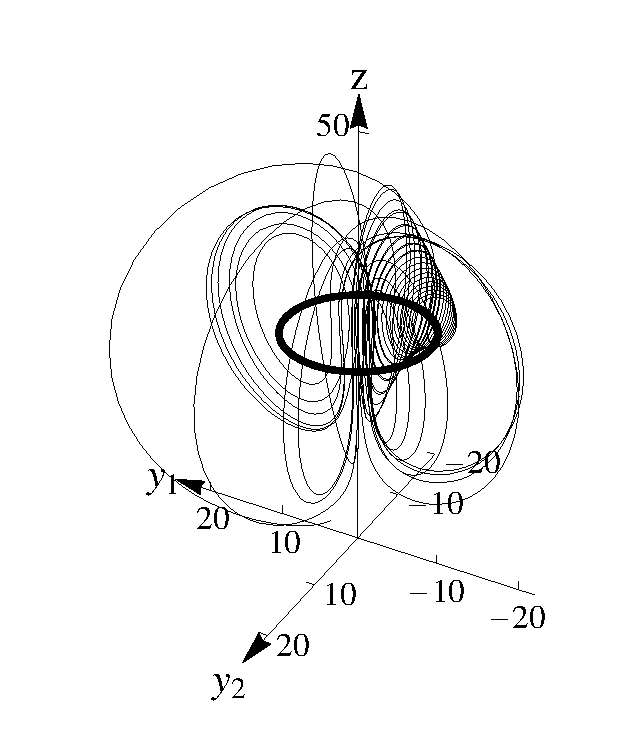
\includegraphics[width=0.33\textwidth]{Fullspace}%
~~~~~~~~
(b)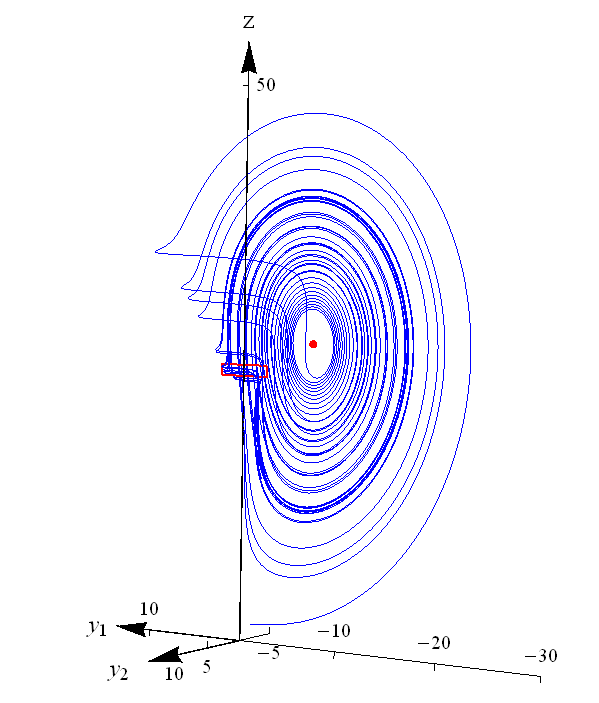
\includegraphics[width=0.32\textwidth]{RedTrajNoPlane1}%
 \end{center}
 \caption{\label{fig:Fullspace}
(color online).
(a) \CLe\ \refeq{eq:CLeR} exhibit a strange attractor for parameter
values \refeq{SiminosPrmts}, here projected on the $\{y_1,y_2,z\}$ axes.
(thin line/blue) A segment of generic finite time trajectory.
(thick line/red)
$\REQV{}{1}$, the only \reqv.
%
% Former {CLEreduced} \label{fig:RedTrajNoPlane1}
(b) The same strange attractor plotted in the symmetry-\reducedsp\
% with initial point
%$(x_1, x_2, y_1, y_2, z) = (1, 2, 3, 1, 2)$
slice \refeq{PCsectQ}, defined by the group tangent $\sliceTan{}$ whose
choice is explained in \refeq{exmplTempl}. In the \reducedsp\ \reqv\
$\REQV{}{1}$ is reduced to \eqv\ $\EQV{1}$. Note, however, the
semicircular jumps in the reduced flow. These are analyzed in
\refsect{sec:singul}. For a blow-up of the jump indicted by the small
rectangle (red), see \reffig{fig:singpass}\,(a).
 }%
 \end{figure}

We shall illustrate symmetry reduction by applying it to the
5-dimensional \cLe\rf{GibMcCLE82}
\bea
	\dot{x}_1 &=& -\sigma x_1 + \sigma y_1
\,,\qquad\qquad\qquad
	\dot{x}_2 \,=\, -\sigma x_2 + \sigma y_2
\continue
	\dot{y}_1 &=& (r_1-z)\, x_1  - ~y_1 - e y_2
\,,\qquad\;
	\dot{y}_2 \,=\, (r_1-z)\, x_2 + e y_1 - ~y_2
\label{eq:CLeR}\\
	\dot{z}~ &=& -b z + x_1 y_1 + x_2 y_2
\,.
\nnu
\eea
In all numerical calculations that follow we shall set the
parameters to \refref{SiCvi10} values,
\beq
r_1=28,\; b={8}/{3},\;
\sigma=10,\quad \mbox{and}  \quad e={1}/{10}
\,,
\ee{SiminosPrmts}
for which the flow exhibits a strange attractor,
\reffig{fig:Fullspace}\,(a).
\CLe\ are a simple example of a dynamical system
with a continuous (but no discrete) symmetry.
They are equivariant \refeq{eq:FiniteRot} under \SOn{2} rotations by
	\ifarticle  %submission version
\bea
\LieEl(\gSpace)
    &=&
\exp{({\gSpace} \cdot \Lg)}
	 \,=\,
  \left(\barr{ccccc}
  \cos \gSpace  & \sin \gSpace  & 0 & 0 & 0 \\
 -\sin \gSpace  & \cos \gSpace  & 0 & 0 & 0 \\
 0 & 0 &  \cos \gSpace & \sin \gSpace   & 0 \\
 0 & 0 & -\sin \gSpace & \cos \gSpace   & 0 \\
 0 & 0 & 0             & 0              & 1
    \earr\right)
\continue
\Lg &=&
   \left(\barr{ccccc}
    0  &  1 & 0  &  0 & 0  \\
   -1  &  0 & 0  &  0 & 0 \\
    0  &  0 & 0  &  1 & 0  \\
    0  &  0 &-1  &  0 & 0 \\
    0  &  0 & 0  &  0 & 0
    \earr\right)
% \,.
\label{CLfRots}
\eea
    \else  %web version
\bea
\LieEl(\gSpace)
    &=&
\exp{({\gSpace} \cdot \Lg)}
	 \,=\,
  \left(\barr{ccccc}
  \cos \gSpace  & \sin \gSpace  & 0 & 0 & 0 \\
 -\sin \gSpace  & \cos \gSpace  & 0 & 0 & 0 \\
 0 & 0 &  \cos \gSpace & \sin \gSpace   & 0 \\
 0 & 0 & -\sin \gSpace & \cos \gSpace   & 0 \\
 0 & 0 & 0             & 0              & 1
    \earr\right)
\,,\qquad \Lg \,=\,
   \left(\barr{ccccc}
    0  &  1 & 0  &  0 & 0  \\
   -1  &  0 & 0  &  0 & 0 \\
    0  &  0 & 0  &  1 & 0  \\
    0  &  0 &-1  &  0 & 0 \\
    0  &  0 & 0  &  0 & 0
    \earr\right)
% \,.
\label{CLfRots}
\eea
	\fi
(for group-theoretical notation, see \refappe{sec:SymmDyn}). The group is
1\dmn\ and compact, its elements parameterized by $\gSpace \mbox{ mod }
2\pi$. The fixed-point subspace \refeq{dscr:InvPoints} is the $z$-axis.
The velocity \refeq{eq:CLeR} at a point on the $z$-axis points only in
the $z$-direction and so the trajectory remains on the $z$-axis for all
times. The action of \SOn{2}\ thus decomposes the  \statesp\ into $m=0$
invariant subspace ($z$-axis) and  $m=1$ subspace of multiplicity
2. Locally, at \statesp\ point $\ssp$, the infinitesimal action of the
group is given by the group tangent field $\groupTan(\ssp) = \Lg \ssp =
(x_2,-x_1,y_2,-y_1,0)$, with the flow induced by the group action normal
to the radial direction in the $(x_1,x_2)$ and $(y_1,y_2)$ planes, while
the $z$-axis is left invariant.


\section{\Mframes}
    \label{sec:frame}
% former siminos/froehlich/slice/frame.tex 2011-01-13

Suppose you are observing turbulence in a pipe flow, or your
defibrillator has a mesh of sensors measuring electrical currents that
cross your heart, or you have a precomputed pattern, and are sifting
through the data set of observed patterns for something like it. Here you
see a pattern, and there you see a pattern that seems much like the first
one. How `much like the first one?' Think of the first pattern
(represented by a point {\slicep} in the \statesp\  \pS) as a
`template'\rf{rowley_reconstruction_2000,rowley_reduction_2003} or a
`reference state' and use the symmetries of the flow to slide and rotate
the `{\template}' until it overlays the second pattern (a point $\ssp$ in
the \statesp), \ie, act with elements of the symmetry group \Group\ on
the {\template} $\slicep \to \LieEl(\gSpace)\,\slicep$ until the
distance between the two patterns
\beq
|\ssp - \LieEl(\gSpace)\,\slicep|
    = |\sspRed - \slicep|
\label{minDistance0}
\eeq
is minimized. Here $\sspRed$ is the point on the group orbit of $\ssp$
(the set of all points that $\ssp$ is mapped to under the group
actions),
\beq
\ssp=\LieEl(\gSpace)\,\sspRed
	\,,\qquad
\LieEl \in \Group
\,,
\ee{sspOrbit}
closest to the {\template} {\slicep}, the Lie group element
$\LieEl=\LieEl(\gSpace)\propto\exp{({\gSpace} \cdot \Lg)}$ is
parameterized by angles $\gSpace =
(\gSpace_1,\gSpace_2,\cdots\gSpace_N)$, and the distance is an invariant
of the symmetry group, $|\LieEl\ssp|^2=|\ssp|^2$. We assume that \Group\
is a subgroup of the group of orthogonal transformations
$\On{d}$, and measure
distance $|\ssp|^2=\braket{\ssp}{\ssp}$ in terms of the Euclidean inner
product
\( %beq
\braket{x}{y} = \sum_i^d {x}_i y_i
%    \,,\; %\qquad
% x, y \in \pS \subset \reals^d
	\,.
\) %\ee{innerR}
Its Lie algebra {generators} $\Lg_a$ \refeq{FiniteRot} are $N$
linearly independent $[d\!\times\!d]$ antisymmetric matrices acting
linearly on the {\statesp} vectors $\ssp \in \pS \subset \reals^d$.

If the \statesp\ is a normed function space,
\( %\beq
\braket{g}{f} = \int dx \, {g}(x) f(x)
\,,
\) %\ee{innerL2}
one customarily measures distance between two patterns in the $L^2$ norm
$|f|^2 = \braket{f}{f}$. In computations, spatially extended functions are
represented by discrete meshes or finite basis sets, within a (possibly
large) finite-dimensional \statesp\  $\pS \subset \reals^d$. An example
is representation of a dissipative PDE by truncating the Fourier basis
\refeq{FourierExp} to a finite number of modes.

The minimal distance satisfies the extremum conditions
\[ %beq
\frac{\partial ~~}{\partial \gSpace_a} |\ssp - \LieEl\slicep|^2
   =
\braket{\sspRed - \slicep}{\sliceTan{a}}
   = 0
    \,,\qquad
	  \sliceTan{a} = \Lg_a \slicep
\,.
\] % ee{PCsectQ0}
By the antisymmetry of the Lie algebra generators we have
$\braket{\slicep}{\sliceTan{a}} = \braket{\slicep}{\Lg_{a}\slicep}=0$, so
we can replace $\sspRed - \slicep \to \slicep$, and the
`moving frame' transformation
parameters $\gSpace$ which map the state $\ssp$ to $\sspRed$, the group
orbit point closest to the {\template} $\slicep$, are determined by
\beq
\braket{\sspRed}{\sliceTan{a}} =0
    \,,\qquad
\sspRed = \LieEl(\gSpace)\,\ssp
\,.
\ee{PCsectQ}
The closest group orbit points thus lie in a $(d\!-\!N)$\dmn\ hyperplane
$\pSRed = \pS/\Group$, the set of vectors $\sspRed \in  \pSRed$
orthogonal to the {\template} tangent space spanned by tangent vectors
$\{\sliceTan{1},\cdots,\sliceTan{N}\}$
\beq
\sspRed_1\sliceTan{a,1} + \sspRed_2\sliceTan{a,2}
  + \cdots + \sspRed_d\sliceTan{a,d} = 0
\,.
\ee{hyperpl}
In what follows we shall refer to this hyperplane as a \emph{slice,} and
to  \refeq{PCsectQ} as the \emph{slice conditions}. Slice so defined is
a particular case of symmetry reduction by transverse sections of group
orbits\rf{FelsOlver98,FelsOlver99,OlverInv} that can be traced back to
Cartan's \mframes\rf{CartanMF}. `Moving frame' refers to the action
$\LieEl(\gSpace)$ that brings a \statesp\ point \ssp\ into the slice.


In the choice of the {\template} one should avoid solutions
that belong to the invariant or partially symmetric subspaces; for such
choices $\Lg_{a}\slicep=0$, and some or all $\sliceTan{a}$ vanish identically
and impose no slice conditions. The {\template} $\slicep$ should be a
generic \statesp\ point in the sense that its group orbit has the full
$N$ dimensions of the group \Group. In particular, even though the
simplest solutions (laminar, \etc) often capture important physical
features of a flow, most \eqva\ and short \po s have nontrivial
symmetries and thus are not suited as choices of symmetry-reducing
{\template s}.
It should also be emphasized that in general a {\template} is \emph{not}
a spatially {localized} structure. We are not using translations /
rotations to superimpose a localized, `solitonic' solution over a
localized {\template}. In a strongly nonlinear, turbulent flow a good
{\template} is typically a nontrivial global solution.

In summary: the minimum distance condition, combined with the Euclidean
norm, says that the point $\sspRed$ in the group orbit of $\ssp$ closest
to the {\template} $\slicep$ lies in a \emph{slice}, a {\em hyperplane}
normal to the group action tangent space $\sliceTan{}$, for any \statesp\
point $\ssp \in \pS$. {\em Symmetry reduction} by the \mframes\ is a
precise rule for how to pick a unique point \sspRed\ for each such
symmetry equivalence class, and compute the \emph{moving frame}
transformation $\ssp =\LieEl(\gSpace)\, \sspRed$ that relates the full
\statesp\ point  $\ssp \in \pS$ to its symmetry reduced representative
$\sspRed \in \pSRed$.


\subsection{Computing the moving frame rotation angle}
\label{exam:CLErotAngle}

															\toCB
The idea of reducing a flow with Lie-group structure to a system of a
smaller dimension dates back to Lie, Poincar\'e, and Cartan.
Time-evolution and symmetry group actions foliate the \statesp\ into
$(N\!+\!1)$\dmn\ submanifolds: Given a state (a \statesp\ point $\ssp(0)$
at time $\tau=0$), we can trace its  1\dmn\ trajectory $\ssp(\tau)$ by
integrating its equations of motion, and its $N$\dmn\ group orbit by
acting on it with the symmetry group \Group. Locally, a continuous time
flow can be reduced by a \PoincSec; a slice does the same for local
neighborhoods of group orbits.

To show how the rotation into the \slice\ is computed, consider first the
\cLe. Substituting the \SOn{2}\ Lie algebra
generator and a finite angle \SOn{2} rotation \refeq{CLfRots} acting on a
5\dmn\ \statesp\ into the slice condition \refeq{PCsectQ}
yields
\(\braket{\ssp}{\sliceTan{}}\cos\gSpace
    +\braket{\groupTan_{}(\ssp)}{\sliceTan{}} \sin\gSpace
= 0
\,,
\)
and the explicit formula for frame angle $\gSpace$:
\bea
\tan\gSpace &=&
   - \, {\braket{\ssp}{\sliceTan{}}}/
          {\braket{\groupTan_{}(\ssp)}{\sliceTan{}}}
\,.
\label{SL:CLEsliceRot}
\eea
The dot product of two tangent fields in \refeq{SL:CLEsliceRot} is a
sum of inner products weighted by Casimirs \refeq{QuadCasimir},
\beq
\braket{\groupTan(\sspRed)}{\groupTan(\slicep)}
   = \sum_m C_2^{(m)} {\sspRed}_i\, \delta_{ij}^{(m)} \slicep_j
\,.
\ee{braket}
For \cLe\
$\ssp = (x_1,x_2,y_1,y_2,z)$,
$\slicep = (x_1',x_2',y_1',y_2',z')$,
and the moving frame condition \refeq{SL:CLEsliceRot} yields
\beq
\tan\gSpace =
- \, \frac{x_1 x_2'-x_2 x_1'+y_1 y_2' -y_2 y_1'}
       {x_1 x'_1+x_2 x'_2+y_1 y'_1+y_2 y'_2}
\,.
\ee{braketCL}
This formula is particularly simple, as in the \cLe\
example the group acts only through $m=0$ and $m=1$ representations
(in the Fourier mode labeling of \refeq{SO2irrepAlg-Lg}).

Consider next the general form \refeq{SO2irrepAlg-m} of action of an
$\SOn{2}$ symmetry on arbitrary Fourier coefficients of a spatially
periodic function \refeq{FourierExp}. Substituting this into the slice
condition \refeq{PCsectQ} and using \refeq{SO2irrepAlg-m} we find that
    \PC{RECHECK! and prettify this formula}
\bea
\braket{e^{\gSpace \Lg}\ssp}{\groupTan(\slicep)}
=\braket{\ssp}{\sum\limits_m \left(\cos(-m\gSpace) \id^{(m)}
     +\sin(-m\gSpace) \frac{1}{m}\Lg^{(m)}\right) \sliceTan{}}
\continue
=\sum\limits_m
   \left(
    \braket{\ssp}{\Lg^{(m)} \slicep} \cos(m\gSpace)
  - \braket{\ssp}{\id^{(m)} \slicep} \sin(m\gSpace)
   \right)
   =0
\,.
\label{eq:so2sing}
\eea
This is a polynomial equation, with coefficients determined by
$\braket{\ssp}{\Lg^{(m)} \slicep}$ and $\braket{\ssp}{\id^{(m)}\slicep}$,
as we can see by rewriting $\cos(m\gSpace)$, $\sin(m\gSpace)$ as
polynomials of degree $m$ in $\sin(\gSpace)$ and $\cos(\gSpace)$. The
phase $\gSpace$ that rotates $\ssp$ into any of the group-orbit
traversals of the slice hyperplane corresponds to a real root of this
polynomial. In general these phases have to be computed numerically.

As a generic group orbit is a smooth $N$\dmn\ manifold embedded in the
$d$\dmn\ \statesp, several values of $\gSpace$ might be local extrema of
the distance function \refeq{minDistance0}.
Our prescription is to pick the closest \reducedsp\ point as the unique
representative of the entire group orbit. \ie, determine the absolute
minimum or the \emph{infimum} of \refeq{minDistance0}.
For example, group orbits of
\SOn{2}\ are topologically circles, and the distance function
\refeq{minDistance0} has maxima, minima and inflection points as extrema:
if \gSpace\ is a solution of the slice condition \refeq{SL:CLEsliceRot},
so is $\gSpace+\pi$. We can pick the closest by noting that
the local minima have positive curvature,
\beq
\frac{\partial^2}
     {\partial \gSpace^2}
        |\sspRed - \slicep|^2
    =
-  \braket{\sspRed}{\Lg^2\slicep}
\,.
\ee{SO2inflPoint}
It does not matter
whether the group is compact, for example $\SOn{n}$, or noncompact, for
example the Euclidean group $E_2$ that underlies the generation of spiral
patterns\rf{Barkley94}; in either case any group orbit has one or several
locally closest passages to the {\template} state, and generically only
one that is the closest one.
(Here we focus only on continuous symmetries - discrete symmetries that
flows such as the \KS\ and {\pCf} exhibit will also have to be taken into
account\rf{SCD07,HGC08,DasBuchMirror}.)

In summary, we do not have to compute all zeros of the slice condition
\refeq{PCsectQ} - all we care about is the infimum, the zero that
corresponds to the shortest distance \refeq{minDistance0}.
While post-processing of a full \statesp\ trajectory $\ssp(\tau_j)$
requires a numerical (Newton method) determination of the
`moving frame' rotation
$\gSpace(\tau_j)$ at each time step $\tau_j$, the computation is not
as onerous as it might seem, as the knowledge of $\gSpace(\tau_j)$ and
$\groupTan(\sspRed(\tau_j))$
gives us a very good guess for $\gSpace(\tau_{j+1})$. We
can go a step further, and write the equations for the flow restricted to
the \reducedsp\ \pSRed.

\subsection{Dynamics within a slice}
\label{sec:mslices}

Any \statesp\ trajectory can be written in a factorized
form $\ssp(\tau)=\LieEl(\tau)
\sspRed(\tau)$. Differentiating both sides with respect to time and
setting $\velRed={d\sspRed}/{d\tau}$ we find
\(
\vel(\ssp)=\dot{\LieEl} \, \sspRed+\LieEl \, \velRed(\sspRed)
\,.
\)
By the equivariance \refeq{eq:FiniteRot}
\[
\vel=\velRed + \LieEl^{-1} \, \dot{\LieEl} \, \sspRed
\,.
\]
Noting that $\LieEl^{-1}\dot{\LieEl}=e^{-\gSpace \cdot \Lg} \,
\frac{d ~~}{d \, \tau} e^{\gSpace \cdot \Lg}=\dot{\gSpace}\cdot \Lg$,
we obtain the equation for the velocity of the reduced flow:
\beq
\velRed(\sspRed)=\vel(\sspRed)-\dot{\gSpace}(\sspRed)\cdot \groupTan(\sspRed)
\,.
\ee{eq:redVel}
The velocity $\vel$ in the full \statesp\ is thus the sum of the
`angular' velocity \refeq{PC:groupTan1} along the group orbit,
$\dot{\gSpace} \cdot \groupTan(\ssp)$, and the remainder $\velRed$.

Eq. \refeq{eq:redVel} is true for any factorization
$\ssp=\LieEl \sspRed$, and by itself provides no
information on how to calculate $\dot{\gSpace}$. That is attained by
demanding that the reduced trajectory stays within a slice, by imposing
the slice conditions \refeq{PCsectQ}:
\beq
\braket{\vel(\sspRed)}{\sliceTan{a}}
 -\braket{\dot{\gSpace}\cdot \groupTan(\sspRed)}{\sliceTan{a}}=0
\,.
\label{eq:slicecondition}
\eeq
This is a matrix equation in
$\braket{\groupTan_b(\sspRed)}{\sliceTan{a}}$ that one can in
principle\rf{FiSaScWu96} solve for $\dot{\gSpace}_a$. Here we shall
consider only the $\SOn{2}$ case, which has a single group tangent:
\bea
\velRed(\sspRed) &=& \vel(\sspRed)
   -\dot{\gSpace}(\sspRed) \groupTan(\sspRed)
\continue
\dot{\gSpace}(\sspRed) &=& {\braket{\vel(\sspRed)}{\sliceTan{}}}/
               {\braket{\groupTan(\sspRed)}{\sliceTan{}}}
\,.
\label{eq:so2reduced}
\eea
One way to think about this reduction of a flow to a slice is in terms of
Lagrange multipliers (see {Stone and Goldbart}\rf{StGo09}, Sect 1.5 for
intuitive, geometrical interpretation of Lagrange multipliers). The first
equation defines the flow confined to the slice (see
\reffig{fig:Fullspace}\,(b)), and integration of the second,
`reconstruction' equation\rf{Marsd92,MarsdRat94} enables us to track the
corresponding trajectory in the full \statesp. For invariant subspaces
$\dot{\gSpace}=0$, so they are always included within the slice. No
information is lost about the physical flow: if we know one point on a
trajectory, we can hop at will back and forth between the reduced
and the full \statesp\ trajectories, just as we can reconstruct a
continuous trajectory from its \PoincSec s.

\section{\Sset}
	\label{sec:singul}
% former siminos/froehlich/slice/singul.tex 2011-01-13

If  two patterns are close, their group orbits are nearly parallel,
$\braket{\groupTan(\ssp)}{\sliceTan{}} \neq 0$, and a slice is transverse
to all group orbits in an open neighborhood of the {\template} \slicep.
However, globally the \mslices\ always introduces singularities. Two
hyperplanes are associated with  any given {\template} \slicep; the slice
\refeq{PCsectQ}, and the hyperplane of points \sspSing\ such that from
the {\template} vantage point their group orbits are not transverse, but
locally `horizontal,'
\beq
\braket{\groupTan(\sspSing)}{\sliceTan{}}
 =
\braket{\sspSing}{\Lg^2\slicep}
 =0
%\,.
\ee{sliceSingl0}
(for simplicity, in this section we specialize to the  $\SOn{2}$ case).
We shall refer to the $(d\!-\!2)$\dmn\ intersection of the two as the
{\em \sset} $S$,
\beq
\braket{\groupTan(\sspRSing)}{\sliceTan{}}
 =
\braket{\sspRSing}{\Lg^2\slicep}
 =0
\,.
\ee{sliceSingl}
\ES{I cannot see how you go from \refeq{sliceSingl0} to \refeq{sliceSingl}.
Is $\sspSing$ still unreduced space point? How do you bring it to the
slice (if you do)?}
Looking back at \refeq{SO2inflPoint}, we see that $S$ is the locus of
inflection points, a hyperplane through which the curvature of the
distance function changes sign, and a local minimum turns into a local
maximum.  For example, for \cLe\ $\sspRSing =
(x_1^*,x_2^*,y_1^*,y_2^*,z^*)$, $\slicep = (x_1',x_2',y_1',y_2',z')$, and
the 3\dmn\ {\sset} $\sspRSing \in S \subset \pSRed$ is given by vanishing
denominator in \refeq{braketCL}:
\[
0 = {x_1^* x'_1+x_2^* x'_2+y_1^* y'_1+y_2^* y'_2}
\,.
\]
The {\sset}  $S$ is purely an artifact of the choice of a {\template},
and has nothing to do with the dynamics; whenever the full \statesp\
trajectory crosses an {\sset}, it pays it no heed whatsoever.

We next show that the singularity in
the formula \refeq{SL:CLEsliceRot} causes a discontinuous jump in the
moving frame angle $\gSpace$. Consider a full \statesp\ trajectory
$\ssp(\tau)$ that passes through the {\sset} \refeq{sliceSingl} at time
$\sspRSing =\ssp(\tau^*)$, which we shall set to  $\tau^*=0$. At that
instant the moving frame angle $\gSpace$ is formally undefined: the
numerator $\braket{\sspRSing}{\sliceTan{}}$ in \refeq{SL:CLEsliceRot}
vanishes ($\sspRSing$ is in the slice and satisfies the slice condition
\refeq{PCsectQ}), and the denominator
${\braket{\groupTan_{}(\sspRSing)}{\sliceTan{}}}$ vanishes by
\refeq{sliceSingl}. Nevertheless, the trajectory going through the singularity
is well defined, as in the linear approximation the numerator and the
denominator in the moving frame formula \refeq{SL:CLEsliceRot} are given
by
\bea
\braket{\ssp}{\sliceTan{}}
    &=&
\braket{(\sspRSing+\vel(\sspRSing) \, \tau ))}
       {\sliceTan{a}}
    \,=\,  \braket{\vel(\sspRSing)}
       {\sliceTan{a}} \, \tau
	\label{singSetVelo}\\
\braket{\groupTan(\ssp)}{\sliceTan{}}
    &=&
\braket{\groupTan(\sspRSing+\vel(\sspRSing) \, \tau ))}
       {\sliceTan{a}}
    \,=\, \braket{\groupTan(\vel(\sspRSing))}
       {\sliceTan{a}} \, \tau
\,.
\label{singSetSign}
\eea
In other words, the moving frame rotates the \statesp\ point $\ssp$ and
the velocity $\vel(\ssp)$ by the same angle, so either can be used to
compute it. The infimum in the slice condition demands that we pick the
solution with positive curvature \refeq{SO2inflPoint}, so
$\braket{\groupTan(\ssp)}{\sliceTan{}}\geq 0$
for all $\tau$. As the trajectory traverses $\sspRSing$, the time $\tau$
changes the sign from negative to positive; hence we must switch from the
solution $\sspRSing$ to another extremum for which
$\braket{\groupTan(\vel(\sspRSing))}{\sliceTan{}}$ is positive. In the
\cLf\ example there are only two extrema $\{\gSpace,\gSpace+\pi\}$,
so the moving frame angle $\gSpace$ jumps discontinuously by $\pi$.

Within the \reducedsp\  an {\sset} crossing has a dramatic effect: the
\reducedsp\ flow $\sspRed(\tau)$ \emph{jumps} whenever it crosses the
{\sset} $\sspRSing$, by amount that we now compute.
Suppose that a \reducedsp\ trajectory passes through a singularity
$\sspRSing$ at time $\tau=\tau^*$. At
that instant the numerator $\braket{\vel(\sspRSing)}{\sliceTan{a}}$ is
(generically) finite, but as the group tangent of the point $\sspRSing$
lies in the slice, ${\braket{\groupTan_{}(\sspRSing)}{\sliceTan{}}}=0$
by \refeq{sliceSingl}, the denominator in \refeq{eq:so2reduced} vanishes,
and the {\angVel} $\dot{\gSpace}$ shoots off to infinity.
\SF{For the nearby trajectories the numerator is nonzero, but along a
trajectory passing through a singularity doesn't the numerator approach
zero $\gSpace$ approach the angle required to rotate the velocity into
the slice? Hence the infinitely thin delta function}

% 2010-12-20 previously {CLEsingpass}{CLEnearsing2}
 \begin{figure}
 \begin{center}
(a) 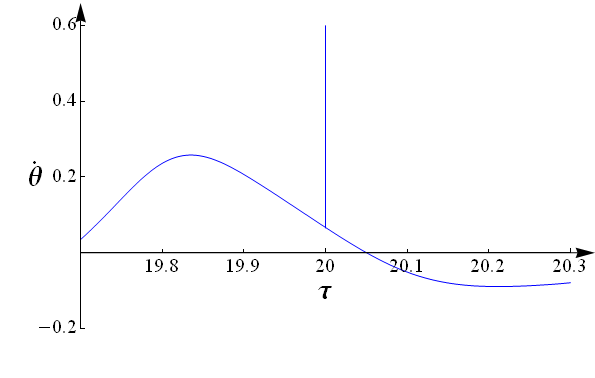
\includegraphics[width=0.35\textwidth]{dthetasing}%
~~
(b) 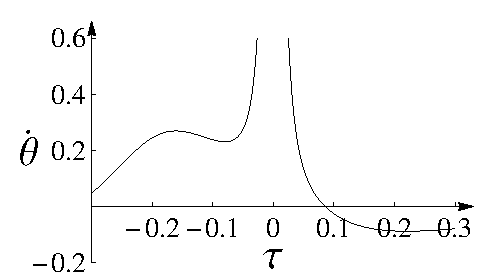
\includegraphics[width=0.35\textwidth]{dthetanearsing}%
 \end{center}
 \caption{\label{fig:dthetasing}
The {\angVel} $\dot{\gSpace}$ for two \cLf\
\reducedsp\ trajectories in a slice defined by the
{\template} $\slicep$ given in \refeq{exmplTempl}:
 (a) As the trajectory $\sspRed(\tau)$ passes through the
singular point  $\sspRSing$ given in \refeq{exmplTempl},
the {\angVel} diverges
$\dot{\gSpace} \to \infty$ as a Dirac delta function.
(b) The {\angVel} for a nearby trajectory going
through $\sspRSing+\delta \ssp$,
$\delta\ssp=(0.01,0,0,0,0)$ exhibits a large
but finite excursion close to the singularity.
 }%
 \end{figure}

As an illustration of such jump, consider a blow-up of the small rectangle indicated
in \reffig{fig:Fullspace}\,(b). Here the {\template}
\bea
\slicep 	&=& (0.887846,-0.150461,0.4,-0.12,0)
	\continue
\sliceTan{} &=& (0.150461,0.887846,0.12,0.4,0)
	\label{exmplTempl} \\
\sspRSing	&=& (-0.889135, -0.0401956, 1.91332, -0.150327, 24.4436)
\nnu
\eea
was reverse-engineered, by picking a point $\sspRSing = \ssp(0)$ from a
segment of the full \statesp\ ergodic trajectory $\ssp(\tau)$ and then
computing \slicep\ such that $\sspRSing$ lies in the {\sset}. As the
trajectory $\sspRed(\tau)$ passes through the $\sspRSing$, the {\angVel}
diverges $\dot{\gSpace} \to \infty$ as a Dirac delta function,
\reffig{fig:dthetasing}\,(a), and the \reducedsp\ trajectory goes through
the inflection \refeq{sliceSingl} and jumps to the $\pi$-rotated extremum
of the distance function, \reffig{fig:singpass}\,(a).

The {\sset} $S$ is the intersection of two hyperplanes: (1) the slice
(infimum of the group-orbit distance to the {\template}), and (2) the
closest inflection in the distance function \refeq{sliceSingl}, and thus
of higher codimension than either. While all group orbits of a  generic
trajectory cross the slice, the trajectory has vanishing probability to
cross the lower-dimensional {\sset} - that is why we had to `engineer'
the slice \refeq{exmplTempl}. However, an ergodic trajectory  might come
arbitrarily close to  $S$ arbitrarily often.
	\PC{This hopefully resolves a long-standing conundrum for Evangelos
        and me. Please CORRECT ME if I am wrong, I'm on thin ice here!}
Such nearby \reducedsp\ trajectories exhibit large {\angVels} $\dot{\gSpace}$,
\reffig{fig:dthetasing}\,(b), and very fast, nearly semi-circular
excursions close to the singularity, \reffig{fig:singpass}\,(a). Which segment
of the group orbit they follow depends on the side from which the
trajectory approached the {\sset}.

% 2011-01-12 previously Figs. {singpass} and {fig:Tesselate}
% In FrCv11.tex replaced by f_1_08_1.png
%{Hyp} %{fig6} and {tr:fig6} in ChaosBook
% \HREF{http://chaosbook.org/overheads/trace/Tesselate.jpg}
 \begin{figure}
 \begin{center}
(a) 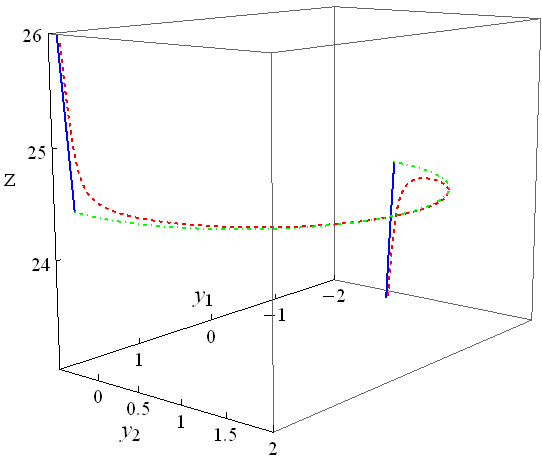
\includegraphics[width=0.32\textwidth]{singpass1}%
~~~~~~~~
(b)~ 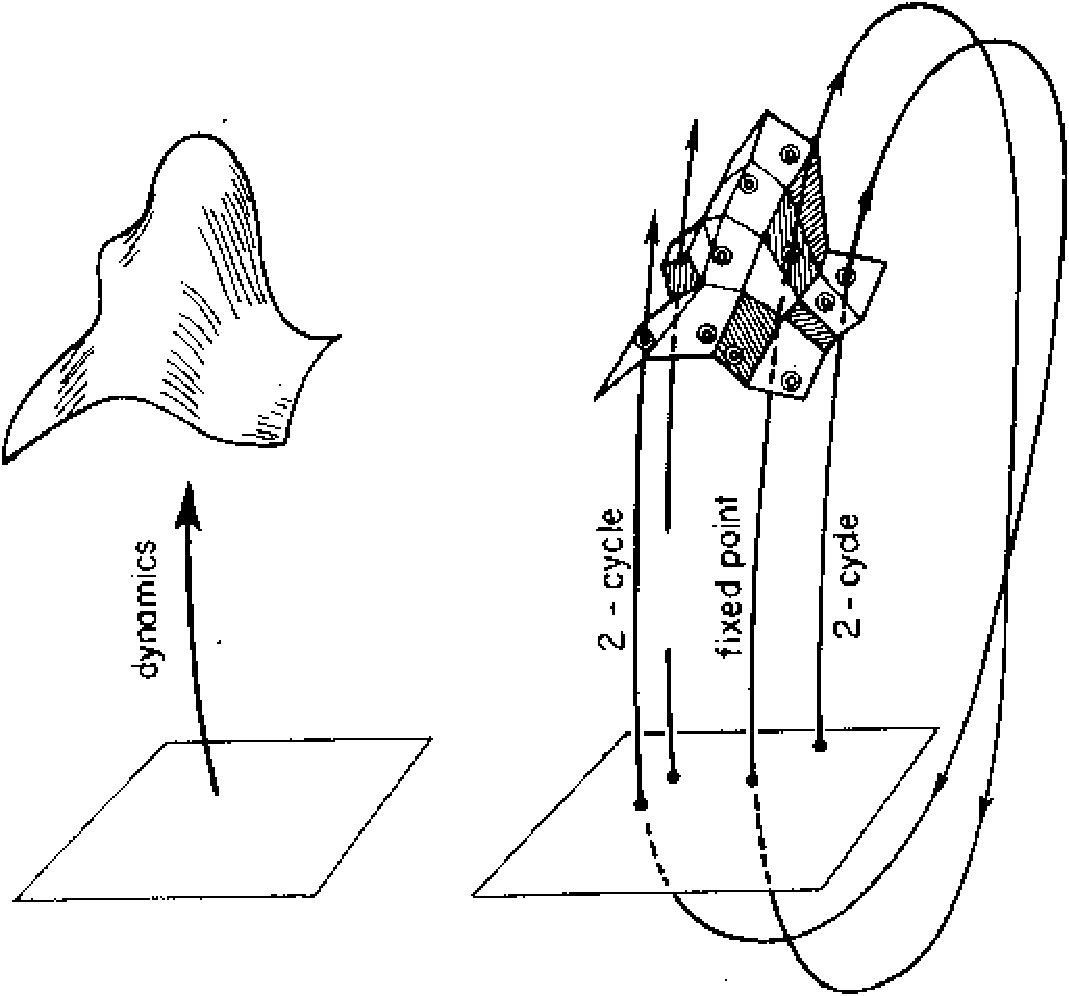
\includegraphics[width=0.40\textwidth]{f_1_08_1}
 \end{center}
 \caption{\label{fig:singpass}
(color online).
(a)
Blow-up of a jump in \reffig{fig:Fullspace}\,(b), indicated by a small
rectangle.
(blue/dotted) A trajectory that passes through the singular point
$\sspRSing$ given in \refeq{exmplTempl}. Note the instantaneous jump in
the trajectory,  caused by the divergence in velocity
(\reffig{fig:dthetasing}\,(a)) as the trajectory traverses the {\sset}.
The neighboring red/dashed trajectory going through $\sspRSing+\delta
\ssp$, $\delta \ssp =(0,0.025,0,0,0)$, makes a rapid transit around the
singularity. The green trajectory is the group orbit of $\sspRSing$
between the two $\gSpace$ that rotate $v(\sspRSing)$ in the slice. Note
also how the red/dashed trajectory begins near the blue/dotted
trajectory, closely follows the green trajectory after the singularity
point, reaches the other side of the blue/dotted arc and then resumes
closely following the blue/dotted trajectory.
(b)
Smooth dynamics  (left frame) tesselated by the skeleton of periodic
points, together with their linearized neighborhoods, (right frame).
Indicated are segments of two 1-cycles and a 2-cycle that alternates
between the neighborhoods of the two 1-cycles, shadowing first one, and
then the other
(from \wwwcb{}).
 }%
 \end{figure}

In summary, whenever a \reducedsp\ trajectory crosses the {\sset}, it
jumps instantaneously and discontinuously to the new distance infimum. We
have shown that these jumps are harmless and theoretically under control.
Nearby trajectories are numerically under control if sufficient care is
taken to deal with large \angVels. But they are an artifact of the
\mslices\ of no dynamical significance, and an uncalled-for numerical
nuisance. We now outline a strategy how to avoid them altogether by a
clever choice of {\template s}.
	\PC{no, not
\HREF{http://en.wikipedia.org/wiki/Infimum}{infinum}
	}


\section{Charting the \reducedsp}
	\label{sec:chart}
% former file siminos/froehlich/slice/chart.tex 2011-01-13

So far, the good news is that for a generic {\template} $\slicep$ (\ie,
any $\slicep$ whose group orbit has the full $N$-dimensions of the
symmetry group \Group), the slice hyperplane \refeq{PCsectQ} cuts across
the group orbit of {\em every} point in the full \statesp\ \pS. But is
this a useful symmetry reduction of the full \statesp? A distant pattern
that is a bad match to a given {\template} will have any number of
locally `minimal' distances, each yet another bad match. Physically it
makes no sense to use a single slice (a set of all group orbit points
that are closest to one given {\template}) globally.

Work on \KS\ and the work of Rowley and
Marsden\rf{rowley_reconstruction_2000} suggests how to proceed: it was
shown in \refrefs{lanCvit07,SCD07} that for turbulent/chaotic systems a
set of Poincar\'e sections is needed to capture the dynamics. The choice
of sections should reflect the dynamically dominant patterns seen in the
solutions of nonlinear PDEs. We propose to construct a global atlas of
the symmetry \reducedsp\ $\pS/\Group$ by deploying both linear slices and
linear Poincar\'e sections across neighborhoods of the qualitatively most
important patterns, taking care that the {\template s} chosen have no
symmetry. Each slice $\pSRed{}^{(j)}$, tangential to one of a finite
number of {\template s}  $\slicep{}^{(j)}$, provides a local chart for a
neighborhood of an important, qualitatively distinct class of solutions
(2-rolls states, 3-rolls states, \etc); together they `Voronoi'
tessellate  the curved manifold in which the reduced strange attractor is
embedded by a finite set of hyperplane
tiles\rf{rowley_reconstruction_2000,RoSa00}. This is the symmetry-reduced
generalization of the idea of {\statesp\ tessellation} by a set of
periodic-orbits, so dear to a professional cyclist,
\reffig{fig:singpass}\,(b).

So how do we propose to implement this tessellation?

The physical task is to, for a given dynamical flow, pick a set of
qualitatively distinct {\template s} whose slices are locally tangent to
the strange attractor. A `slice' is a purely group-theoretic, linear
construct, with no reference to dynamics; a given {\template}
$\slicep{}^{(1)}$ defines the associated slice $\pSRed$, a
($d\!-\!1$)\dmn\ tangent hyperplane (for simplicity, in this section we
specialize to the $\SOn{2}$ case). Within it, there is a ($d\!-\!2$)\dmn\
{\sset} \refeq{sliceSingl}. If we pick another {\template} point
$\slicep{}^{(2)}$, it comes along with its own slice and {\sset}. Any
neighboring pair of $(d\!-\!1)$\dmn\ slices intersects in a `ridge'
(`boundary,' `edge'), a $(d\!-\!2)$\dmn\ hyperplane, easy to compute. All
intersections of slices, ridges and {\sset s} contain the fixed-point
subspace $\pS_\Group$. A global atlas so constructed should be sufficiently
fine-grained that we never hit any {\sset} singularities. The {\sset}s
should be eliminated by requiring that they lie either on the far sides
of the slice-slice intersections, or elsewhere where the strange
attractor does not tread. Each `chart' or `tile,' bounded by ridges to
neighboring slices, should be sufficiently small so that the {\sset} is
nowhere within the part of the slice explored by the strange attractor.

Follow an ant as it traces out a symmetry-reduced trajectory
$\sspRed{}^{(1)}(\tau)$, confined to the slice $\pSRed{}^{(1)}$. The
moment $\braket{\sspRed{}^{(1)}(\tau)}{\sliceTan{}{}^{(2)}}$ changes
sign, the ant has crossed the ridge, we symmetry-reduce with respect to
the second slice, and the ant continues its merry stroll within the
$\pSRed{}^{(2)}$ slice. Or, if you prefer to track the  given full
\statesp\ trajectory $\ssp(\tau)$, you compute the moving-frame angle
with respect to each (global) slice, and check to which tile does the
given group orbit belong.

There is a rub, though - you need to pick the phases of neighboring
{\template s} in such way that you minimize the distance from one to the
next as the ant crosses the ridge. This a reflection of the flaw inherent in use
of a linear slice globally: a slice is derived from the Euclidean
notion of distance, but for nonlinear flows the distance has to be
measured curvilinearly, along unstable
manifolds\rf{Christiansen97,DasBuch}. We nevertheless have to stick with tessellation by
linearized tangent spaces, as curvilinear charts seem computationally too
prohibitive. The {\em relative phase} between two
different \reqva\ can be fixed, as proposed in \refref{SCD07}, by the
shortest heteroclinic connection, a rigid bridge from one
neighborhood to the next.



\section{What lies ahead} % Conclusion}
    \label{sec:concl}
% former siminos/froehlich/slice/concl.tex  2011-01-13
% PC 2011-01-05 incorporated concl.tex from the SF article

Many physically important spatially extended and fluid dynamics systems
exhibit continuous symmetries. For example,  excitable
media\rf{ZaZha70,Winfree73,Winfree1980,BaKnTu90,Barkley94}, \KS\
flow\rf{ku,siv,SCD07}, {\pCf}\rf{Visw07b,GHCW07,HGC08,GibsonMovies}, and
pipe flow\rf{Wk04,Kerswell05} are invariant (equivariant) under
combinations of translational (Euclidean), rotational and discrete
symmetries. If a physical problem has a symmetry, one should use it - one
does not want to compute the same solution over and over, all one needs
is to pick one representative solution per each symmetry related
equivalence class. Such procedure is called symmetry reduction.  In this
paper we have investigated symmetry reduction by the \mslices, a linear
procedure particularly simple and practical to implement, and answered
affirmatively the two main questions about the method:
(1) does a slice cut the group orbit of \emph{every} point in the
dynamical \statesp?
(2) can one deal with the {\sset s} that the method necessarily
introduces?

We have shown here that a symmetry-reduced trajectory passes through such
singularities through computable jumps, a nuisance numerically, but cause
to no conceptual difficulty. However, while a slice intersects each group
orbit in a neighborhood of a {\template} only once, extended globally any
slice intersects every group orbit multiple times. So even though every
slice cuts all group orbits, it makes no sense physically to use one
slice (a set of \emph{all} group orbit points that are closest to a given
{\template}) globally. We propose instead to construct a global atlas by
deploying sets of slices and linear Poincar\'e sections as charts of
neighborhoods of the most important (relative) equilibria and/or
(relative) periodic orbits.

Such global atlas should be sufficiently fine-grained so that an
unstable, ergodic trajectory never gets too close to any of the {\sset
s}. Why does this proposal have none of the elegance of, let's say,
Killing-Cartan classification of simple Lie algebras? Why is this
symmetry reduction purely a numerical procedure, rather than an analytic
change of equivariant coordinates to invariant ones? The theory of
\emph{linear} representations of compact Lie groups is a well developed
subject, but role of symmetries in \emph{nonlinear} settings is
altogether another story. It is natural to express a dynamical system
with a symmetry in the symmetry's linear eigenfunction basis (let  us
say, Fourier modes), but for a nonlinear flow different modes are
strongly coupled, and group orbits embedded in such coordinate bases can
be highly convoluted, in ways that no single global linear slice
hyperplane can handle intelligibly.

It should be emphasized that the atlas so constructed retains the
dimensionality of the original problem. The full dynamics is faithfully
retained, we are \emph{not} constructing a lower-dimensional model of the
dynamics. Neighborhoods of unstable \eqva\ and \po s are dominated by
their unstable and least contracting stable eigenvalues and are, for all
practical purposes, low-dimensional. Traversals of the ridges are,
however, higher dimensional. For example, crossing from the neighborhood
of a two-rolls state into the neighborhood of a three-rolls state entails
going through a pattern `defect,' a rapid transient whose precise
description requires many Fourier modes. Nevertheless, the recent
progress on separation of `physical' and `hyperbolically isolated'
covariant Lyapunov
vectors\rf{PoGiYaMa06,ginelli-2007-99,YaTaGiChRa08,TaGiCh09} gives us
hope that the proposed atlas could provide a systematic and controllable
framework for construction of lower-dimensional models of `turbulent'
dynamics of dissipative PDEs.

While it has been demonstrated in \refref{SiCvi10}  that the \mslices,
with a judicious choice of the {\template} and {\PoincSec}, works for a
system as simple as the \cLf, one still has to show that the method can
be implemented for a truly high-dimensional flow. In \refref{SCD07} it
was found that the coexistence of four equilibria, two \reqva\ and a
nested \fixedsp\ structure in an effectively $8$-dimensional \KS\ system
complicates matters sufficiently that no symmetry reduction has been
attempted so far. More importantly, a symmetry reduction of pipe flows, which
due to the translational symmetry have only relative (traveling)
solutions, remains an outstanding challenge\rf{ACHKW11}.

	%\begin{acknowledgments}
	\medskip
	\noindent{\bf Acknowledgments}
We sought in vain Phil Morrison's sage counsel on how to reduce
symmetries, but none was forthcoming - hence this article. We are
grateful to
D.~Barkley,
W.-J.~Beyn,
C.~Chandre,
K.A.~Mitchell,
B.~Sandstede,
R.~Wilczak,
and in particular E.~Siminos and R.L.~Davidchack
for spirited exchanges.
S.F. work was supported by the National Science Foundation grant
DMR~0820054 and a Georgia Tech President's Undergraduate Research Award.
P.C. thanks Glen Robinson Jr. for support. 	
	%\end{acknowledgments}
\appendix
\section{Symmetries of dynamics}
	\label{sec:SymmDyn}
% former file siminos/froehlich/slice/symm.tex 2011-01-12

In this Appendix we review a few basic facts about dynamics and
symmetries. We follow notational conventions of
Chaosbook.org\rf{DasBuch}, to which the reader is referred to for a more
extensive discussion of dynamics and symmetries.

If a pipe is rotated around its axis or translated, the shifted and
rotated state of the fluid is a physically equivalent solution of
the Navier-Stokes equations. Such rotations and translations
are examples of continuous symmetries. On the level of equations of
motion, one says that a flow $\dot{x}= \vel(x)$ is \emph{equivariant}
under a coordinate transformation $\LieEl$ if
\beq
\vel(x)=\LieEl^{-1}\vel(\LieEl \, x)
\,.
\ee{eq:FiniteRot}
The totality of elements
$\LieEl$ forms \Group, the {\em symmetry group} of the flow.
An element of a compact Lie group $\Group \subset \On{d}$ that is
continuously connected to the identity can be parametrized as
\beq
\LieEl(\gSpace)=e^{{\gSpace} \cdot \Lg }
    \,,\qquad
\gSpace \cdot \Lg = \sum_{a=1}^N \gSpace_a \Lg_a
\,,
\ee{FiniteRot}
where $\gSpace \cdot \Lg $ is a \emph{Lie algebra} element, $\gSpace =
(\gSpace_1,\gSpace_2,\cdots\gSpace_N)$ are the parameters (`phases,'
`angles,' `shifts') of the transformation, and the $\Lg_a$ are a set of
$N$ linearly independent $[d\!\times\!d]$ antisymmetric matrices acting
linearly on the {\statesp} vectors. A spatial transformation induced by
infinitesimal variations of group phases
$
\LieEl(\delta \gSpace) \simeq 1 + \delta \gSpace \cdot \Lg
\,.
$ %\ee{eq:infinitesimal}
is
\beq
\delta {\ssp} = \delta \gSpace \cdot \groupTan(\ssp)
\,,
\ee{PC:groupTan0}
where the $N$ vectors
\beq
 \groupTan_{a}(\ssp) = \Lg _{a} \ssp
    \,,\qquad
 a=1,2,\cdots,N,
\ee{PC:groupTan}
span the group tangent space at $\ssp$. We use $\groupTan_a(\ssp)$
notation (rather than $\Lg_{a}\ssp$) to emphasize that the group action
induces a \emph{tangent field} at $\ssp$.
A transformation induced by infinitesimal
time-dependent variations \refeq{PC:groupTan0} of group phases
can be thought of as an `{\angVel},'
$\delta \gSpace_a = \timeStep \, \dot{\gSpace_a}$ is
\beq
\dot{\ssp} = \dot{\gSpace} \cdot \groupTan(\ssp)
\,.
\ee{PC:groupTan1}

The {tangent field} is of dimension $N$, as long as the point $\ssp$ does
not belong to a fixed-point subspace. Points in the \emph{fixed-point
subspace}  $\pS_\Group$ are fixed points of the full group action. They
are called \emph{invariant points},
\beq
\pS_\Group = \Fix{\Group} =
   \{ \ssp \in \pS : {g} \, \ssp = \ssp \mbox{ for all } g \in \Group \}
\,,
\ee{dscr:InvPoints}
or, infinitesimally,  $\Lg_{a}\ssp=0$. If a point is an invariant point
of the symmetry group, by equivariance the velocity at that point is also
in $\pS_\Group$, so the trajectory through that point will remain in
$\pS_\Group$. $\pS_\Group$ is disjoint from the rest of the {\statesp}
since no trajectory can ever enter or leave it.

Any representation of a compact group $\Group$ is fully reducible. The
invariant tensors constructed by contractions of $\Lg_a$ are useful in
identifying irreducible representations. The simplest such invariant is
\beq
{\Lg} \cdot \Lg = - \sum_m C_2^{(m)} \, \id^{(m)}
\,,
\ee{QuadCasimir}
where $C_2^{(m)}$ is the quadratic Casimir for irreducible representation
labeled $m$, and $\id^{(m)}$ is the identity on the irreducible
subspace $m$, 0 elsewhere. For compact groups $C_2^{(m)}$ are strictly
nonnegative. $C_2^{(m)} =0$ if $m$ is an invariant subspace.

    %
% \subsection{\SOn{2} irreducible representations.}
%   \label{exam:SO2irrepst}
    %
The simplest example of a Lie group is given by the action of \SOn{2} on
a smooth function $u(\gSpace + 2\pi) = u(\gSpace)$ periodic on interval
$[-\pi,\pi]$. Expand $u$ as a Fourier series
\beq
u(\gSpace) = \frac{a_0}{2} + \sum_{m=1}^\infty \left(
a_m \cos m \gSpace + b_m \sin m \gSpace
                               \right)
\,.
\ee{FourierExp}
The matrix representation of the \SOn{2}\ action
$\LieEl(\gSpace') u(\gSpace) = u(\gSpace+\gSpace')$
on the Fourier coefficient pair
$(a_m,b_m)$ is
	\ifarticle  %submission version
\bea
\LieEl^{(m)}(\gSpace')
    &=& \exp{\left({\gSpace} \cdot \Lg^{(m)}\right)}
	\,=\,
   \left(\barr{cc}
 ~\cos m \gSpace'  & \sin m \gSpace' \\
 -\sin m \gSpace'  & \cos m \gSpace'
    \earr\right)
\continue
&=&
 \cos m \gSpace' \id^{(m)}
  + \sin m \gSpace'\, \frac{1}{m} \Lg^{(m)}
\,.
\label{SO2irrepAlg-m}
\eea
    \else  %web version
\bea
\LieEl^{(m)}(\gSpace')
    &=& \exp{\left({\gSpace} \cdot \Lg^{(m)}\right)}
	\,=\,
   \left(\barr{cc}
 ~\cos m \gSpace'  & \sin m \gSpace' \\
 -\sin m \gSpace'  & \cos m \gSpace'
    \earr\right)
\,=\,
 \cos m \gSpace' \id^{(m)}
  + \sin m \gSpace'\, \frac{1}{m} \Lg^{(m)}
\,.
\label{SO2irrepAlg-m}
\eea
	\fi
Here
\beq
 \Lg^{(m)} =   \left(\barr{cc}
    0  &  m  \\
   -m  &  0
    \earr\right)
%\,.
\label{SO2irrepAlg-Lg}
\eeq
is the Lie algebra generator and $\id^{(m)}$ is the identity
on the irreducible subspace labeled $m$, 0 elsewhere. The \SOn{2}\ group
tangent $\groupTan(u)$ to \statesp\ point $u$ is
\beq
 \groupTan(u) = \sum_{m=1}^\infty \groupTan^{(m)}(u)
    \,,\qquad
 \groupTan^{(m)}(u)
\,=\, m \,\left(\barr{c}
   ~b_m  \\
   -a_m
    \earr\right)
\,.
\ee{u:x:tang}


\section{Singularities of $\SOn{2} \times \SOn{2}$}
	\label{sec:singulProd}
% former file siminos/froehlich/slice/singulProd.tex 2011-01-13

Two groups \Group\ and $H$ can be combined into the {product group}
$\Group \times H$, whose elements are pairs $(\LieEl,h)$, where $\LieEl$
belongs to \Group, and $h$ belongs to $H$, with the group multiplication
rule
\(
(\LieEl_1,h_1)(\LieEl_2,h_2)=(\LieEl_1 \LieEl_2,h_1 h_2)
\,.
\)
Some important fluid-dynamical flows exhibit continuous symmetries which
are the products of $\SOn{2}$ groups, each of which acts on a subset  of
the {\statesp} coordinates. The \KS\ equations\rf{ku,siv},
{\pCf}\rf{Visw07b,GHCW07,HGC08,HalcrowThesis}, and pipe
flow\rf{Wk04,Kerswell05} all have continuous symmetries of this form.

Let $\Group \times H$ be a Lie group with two sets of infinitesimal
generators, $\Lg_1$ and $\Lg_2$, such that the $\Lg_1$ acts only on the
$(a)$ coordinates ($e^{\gSpace_1 \Lg_1} \,
(a,b)=(e^{\gSpace_1\Lg_1}a,b)$), or, infinitesimally,
$\Lg_1(a,b)=(\Lg_1 a,0)$, and $\Lg_2$ acts only on the $(b)$ coordinates,
$\Lg_2(a,b)=(0,\Lg_2 b)$. Taken together, $\Lg_1 \Lg_2(a,b) = \Lg_2
\Lg_1(a,b) = (0,0) $ for all $(a,b)$, so $\Lg_1 \Lg_2=0$.

For simplicity, we now specialize to the  $\SOn{2} \times \SOn{2}$ case.
Suppose we are rotating a trajectory $\ssp(\tau)$ into the slice normal
to the group tangents at $\slicep$. Using the slice condition
\refeq{PCsectQ} yields
$\braket{\vel(\sspRed)}{\sliceTan{1}}-\dot{\gSpace_1} \braket{
\groupTan_1(\sspRed)}{\sliceTan{1}}-\dot{\gSpace_2} \braket{
\groupTan_2(\sspRed)}{\sliceTan{1}}=0$. We have
$\braket{\groupTan_2(\sspRed)}{\sliceTan{1}}=0$ since $\Lg_1 \Lg_2=0$,
leaving us with the equation for $\dot{\gSpace_1}$,
\beq
\dot{\gSpace_1}=     {\braket{\vel(\sspRed)}{\sliceTan{1}}} /
                     {\braket{\groupTan_1(\sspRed)}{\sliceTan{1}}}
\,,
\eeq
and similarly for $\dot{\gSpace_2}$, the same as \refeq{eq:so2reduced}
for the rotation group consisting of only the rotations generated by
either $\Lg_1$ or $\Lg_2$.  This means a point being singular depends
only on whether or not it is singular in either of the slices normal to
only one of the group tangents, breaking up the problem of determining if
a point is singular into the same problem for each of the $\SOn{2}$
separately. In \refsect{sec:singul} we described what happens to the
\reducedsp\ trajectory as it passes through singularity of a single
$\SOn{2}$ symmetry group. Using this result we can handle the
singularities for the product of arbitrarily many $\SOn{2}$.


% \bibliographystyle{model3-num-names}	% CNSNS, gave error after 25 or so refs.
\bibliographystyle{elsarticle-num}  %default style
\bibliography{../../bibtex/siminos}

\ifboyscout
\newpage
    \input ./flotsam
\fi

\end{document}
%
% ****** End of file FrCv11.tex ******
